\section{Theoretische Grundlagen}

    \subsection{Zielsetzung}

        \noindent In diesem Versuch werden allgemein Relaxionsverhalten am Beispiel 
        eines RC-Kreises untersucht.

    \subsection{Allgemeine Relaxionsgleichung}

        \noindent Eine Relaxion beschreibt das Verhalten wenn ein System angeregt wird und dann wieder nicht-oszillatorisch in seinen 
        Ausgangszustand zurückkehrt.\\ Die Geschwindigkeit mit dem dies passiert ist die Ableitung der physikalischen Größe $A$. Diese ist meist 
        proportional zur aktuellen Auslenkung vom Ausgangszustand der wieder bei $A(\infty)$ erreicht wird:

        \begin{equation}
            \frac{\symup{d}A}{\symup{d}t}=c[A(t)-A(\infty)]
            \label{eqn:1}
        \end{equation}

        \noindent Die Integration dieser Gleichung:

        \begin{equation*}
            \int_{A(0)}^{A(t)} \frac{\symup{d}A'}{A' - A(\infty)} = \int_0^t \symup{d}t'
        \end{equation*}

        \noindent liefert

        \begin{equation*}
            \text{ln} \frac{A(t) - A(\infty)}{A(0) - A(\infty)} = ct
        \end{equation*}

        \noindent oder

        \begin{equation}
            A(t) = A(\infty) + [A(0) - A(\infty)] \text{e}^{ct} . 
            \label{eqn:2}
        \end{equation}

        \noindent Hier muss $c < 0$ sein damit $A(t)$ konvergiert.

    \subsection{Entladevorgang im RC-Kreis}

        \noindent Das Standardbeispiel für Relaxionsverhalten in der Physik sind das Aufladen und Entladen eines Kondensators über einen 
        Widerstand (siehe Abbildung \ref{img:A_und_e}).

        \begin{figure}
            \centering
            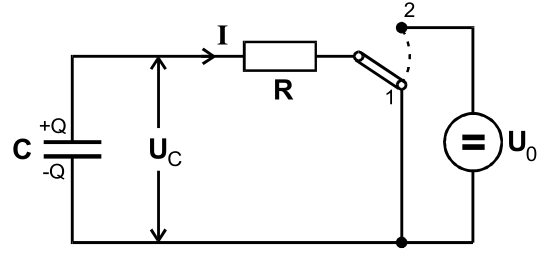
\includegraphics[width=0.5\textwidth]{latex/images/Auflade_und_entlade.PNG}
            \caption{Entladung(1) und Aufladung(2) eines RC-Kreises.\protect \cite{V353}.}
            \label{img:A_und_e}
        \end{figure}

        \noindent Zum Entladen wird wie in Abbildung \ref{img:A_und_e} ein Kondensator mit Kapazität $C$ mit der Ladung $Q$ betrachtet.
        Damit ergibt sich die Kondensatorspannung $U_C$ zu:

        \begin{equation}
            U_{\text{C}} = \frac{Q}{C}
            \label{eqn:3}
        \end{equation}

        \noindent damit berechnet sich nach dem ohmschen Gesetz die Stromstärke durch einen Widerstand $R$ zu

        \begin{equation}
            I = \frac{U_{\text{C}}}{R} .
            \label{eqn:4}
        \end{equation}

        \noindent Auf einem Zeitintervall d$t$ ändert sich die Ladung auf dem Kondensator somit um den Wert:

        \begin{equation}
            \text{d}Q = -I \text{d}t
            \label{eqn:5}
        \end{equation}

        \noindent Über die Gleichungen (\ref{eqn:3}), (\ref{eqn:4}) und (\ref{eqn:5}) lässt sich nun eine Differentialgleichung für die 
        Ladung auf dem Kondensator aufstellen:

        \begin{equation}
            \frac{\text{d}Q}{\text{d}t} = - \frac{1}{RC} Q(t).
            \label{eqn:DGL}
        \end{equation}

        \noindent Da die Ladung auf dem Kondensator für große Zeit gegen 0 konvergiert hat die DGL\ref{eqn:DGL} die Form der 
        Gleichung(\ref{eqn:1}).\\ Nach Gleichung(\ref{eqn:2}) ergibt die Integration:

        \begin{equation*}
            Q(t) = Q(0) \text{exp}(-t/RC).
        \end{equation*}

    \subsection{Aufladevorgang im RC-Kreis}

        \noindent Analog zum Entladevorgang lässt sich eine Gleichung für den Aufladevorgang aufstellen. Hier ist der Kondensator über einen 
        Widerstand $R$ an eine Spannungsquelle der Spannung $U_0$ angeschlossen. Die Randbedingungen ergeben sich somit zu:
    
        \begin{equation*}
            Q(0) = 0 \quad \text{und} \quad Q(\infty) = CU_0 
        \end{equation*}

        \noindent Der Aufladevorgang kann somit durch 

        \begin{equation*}
            Q(t) = CU_0(1- \text{exp}(-t/RC))
        \end{equation*}

        \noindent beschrieben werden. Hier wird der Ausdruck $RC$ als Zeitkonstante bezeichnet. Sie gibt an mit welcher Geschwindigkeit der 
        Endzustand wieder erreicht wird, innerhalb des Zeitraums $\Delta T = RC$ verringert sich die Ladung des Kondensators um den Faktor

        \begin{equation*}
            \frac{Q(t = RC)}{Q(0)} = \frac{1}{e} \approx 0,368 .
        \end{equation*}

        \noindent So sind 10 \% des Ausgangswertes nach $\Delta T = 2,3RC$ und 1\% nach $\Delta T = 4,6RC$ erreicht.

    \subsection{Relaxationsphänomene unter Einfluss einer periodischen Auslenkung}

        \noindent Ein mechanisches System unter Einfluss einer Kraft mit sinusförmiger Zeitabhängigkeit lässt sich analog zu einem RC-Kreis mit 
        einer Sinusspannung beschreiben. Daher wird hier als repräsentatives Beispiel weiter ein RC-Kreis auf Relaxationsphänomene untersucht.\\
        Wird die Wechselspannung $U(t)$ durch

        \begin{equation*}
            U(t) = U_0 \text{cos}( \omega t)
        \end{equation*}

        \noindent beschrieben, so ist bei kleiner Kreisfequenz $\omega \ll 1/RC$, die Spannung am Kondensator ungefähr gleich der Wechselspannung.
        Nimmt die Kreisfrequenz jedoch zu, entsteht eine Phasenverschiebung $\varphi$ zwischen den beiden Spannungen und die 
        Kondensatorspannung verliert an Amplitude. Im Folgenden wird nun diese Frequenzabhängigkeit weiter untersucht.

        \begin{figure}
            \centering
            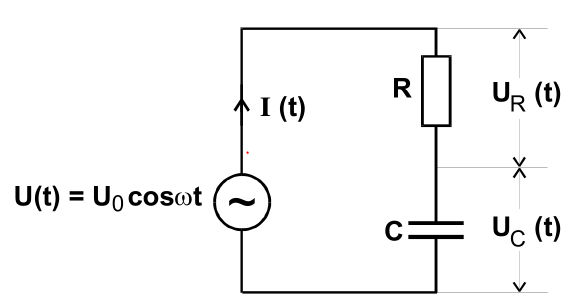
\includegraphics[width=0.5\textwidth]{latex/images/periodische_Auslenkung.PNG}
            \caption{Ein Schaltungsbeispiel zur Untersuchung von Relaxationsphänomenen unter dem Einfluss periodischer Auslenkungen.
            \protect \cite{V353}.}
            \label{img:per_Aus}
        \end{figure}

        \noindent Als Ansatz wird

        \begin{equation}
            U_{\text{C}}(t) = A(\omega) \text{cos}(\omega t + \varphi \{ \omega \} )
            \label{eqn:7}
        \end{equation}

        \noindent gewählt. Insgesamt lässt sich über das Schaltbild aus Abbildung (\ref{img:per_Aus}) mittels des zweiten Kirchhoffschen Gesetz
        folgende Gleichung aufstellen.:

        \begin{equation}
            U(t) = U_R(t) + U_C(t) .
            \label{eqn:7a}
        \end{equation}

        \noindent Einsetzen von Gleichung (\ref{img:per_Aus}) und $U(t)$ ergibt somit:

        \begin{equation*}
            U_0 \text{cos}(\omega t) = I(t)R + A(\omega) \text{cos}(\omega t + \varphi) .
        \end{equation*}

        \noindent Des weiteren kann mittels Gleichung (\ref{eqn:3}) und (\ref{eqn:5}) $I(t)$ durch $U_{\text{C}}$ ausdrücken.

        \begin{equation}
            I(t) = \frac{\text{d}Q}{\text{d}t} = C \frac{\text{d}U_\text{C}}{\text{d}t}
            \label{eqn:9}
        \end{equation}

        \noindent Insgesamt ergibt sich nun also folgende Beziehung:

        \begin{equation}
            U_0 \text{cos}(\omega t) = -A(\omega) R C \text{sin}(\omega t + \varphi) + A(\omega) \text{cos}(\omega t + \varphi) .
            \label{eqn:10}
        \end{equation}

        \noindent Aus Gleichung(\ref{eqn:10}) lässt sich mit $\omega t = \frac{\pi}{2}$ 

        \begin{equation*}
            0 = -\omega R C \text{sin} \left( \frac{\pi}{2} + \varphi \right) + \text{cos} \left( \frac{\pi}{2} + \varphi \right)
        \end{equation*}

        \noindent aufstellen. Daraus folgt mit $\text{sin}(\varphi + \pi /2 = \text{cos}(\varphi))$ und $\text{cos}(\varphi + \pi/2 = - \text{sin}
        (\varphi))$:

        \begin{equation*}
            \frac{\text{sin} \varphi}{\text{cos} \varphi} = \text{tan} \varphi (\omega) = -\omega RC 
        \end{equation*}

        \noindent oder

        \begin{equation}
            \varphi (\omega) = \text{arctan} ( - \omega R C) .
            \label{eqn:11}
        \end{equation}

        \noindent Somit wurde eine Gleichung für die Frequenzabhängigkeit der Phase aufgestellt. Aus dem Verlauf des arctan ist wie vorhergesagt 
        abzulesen, dass bei kleinen Frequenzen die Phasenverschiebung $\varphi$ gegen 0 geht, sich jedoch bei großen Frequenzen $\pi/2$ annährt.
        Eine Phasenverschiebung von $\varphi$ wird genau bei $\omega = 1/RC$ erreicht.\\
        Des weiteren folgt aus Gleichung(\ref{eqn:10}) für $\omega t + \varphi = \frac{\pi}{2}$:

        \begin{equation*}
            U_0 \text{cos}(\frac{\pi}{2} - \varphi) = -A \omega R C ,
        \end{equation*}

        \noindent und somit auch:

        \begin{equation}
            A(\omega) = - \frac{\text{sin} \varphi}{\omega R C} U_0 .
            \label{eqn:12}
        \end{equation}

        \noindent Mittels $\text{sin}^2 \varphi + \text{cos}^2 \varphi = 1$ wird nun aus (\ref{eqn:11}) 

        \begin{equation*}
            \text{sin} \varphi = \frac{\omega R C}{ \sqrt{1 + \omega^2 R^2 C^2} }
        \end{equation*}

        \noindent Daraus folgt mit Gleichung(\ref{eqn:12})

        \begin{equation*}
            A(\omega) = \frac{U_0}{\sqrt{1 + \omega^2 R^2 C^2}} .
        \end{equation*}

        \noindent Somit wurde nun eine Beziehung zwischen der Kondensatorspannung under der Kreisfrequenz der Wechselspannung aufgestellt. Auch 
        hier ist wieder abzulesen, dass für $\omega \rightarrow 0$ die Amplitude der Kondensatorspannung gleich der Amplitude der Wechselspannung ist.
        Ebenso ist abzulesen, dass die Amplitude der Kondensatorspannung für große $\omega$ verschwindet und $A(1/RC) = U_0 / \sqrt{2}$ ist. \\
        Aus diesem Verhalten lässt sich ableiten, dass der RC-Kreis gut als Tiefpass verwendet werden kann.

    \subsection{Der RC-Kreis als Integrator}

        \noindent Für den Fall, dass die Frequenz $\omega \gg 1/RC$ lässt sich zeigen, dass die Kondensatorspannung $U_{\text{C}}$ proportional 
        zu $\int U(t) \text{d}t$ ist. Somit ist der RC-Kreis in der Lage eine Spannung $U(t)$ zu integrieren.\\
        Ausgehend von Gleichung(\ref{eqn:7a}) gilt:

        \begin{equation*}
            U(t) = U_{\text{R}}(t) + U_{\text{C}}(t) = I(t) \cdot R + U_{\text{C}}(t)
        \end{equation*}

        \noindent  Hier wird dann noch $I(t)$ aus Gleichung(\ref{eqn:9}) eingesetzt.

        \begin{equation}
            U(t) = RC \frac{\text{d}U_{\text{C}}}{\text{d}t} + U_{\text{C}}(t)
            \label{eqn:bums}
        \end{equation}

        \noindent Aus der Vorraussetzung, dass $\omega \gg 1/RC $ ist, ergibt sich nun, dass $|U_{\text{c}}| \ll | U_{\text{R}}|$ und 
        $|U_{\text{C}}| \ll |U|$ sind. Somit lässt sich Gleichung(\ref{eqn:bums}) wie folgend annähern:

        \begin{equation*}
            U(t) = RC \frac{\text{d}U_{\text{C}}}{\text{d}t} ,
        \end{equation*}
        
        \noindent oder in integrierter Form:

        \begin{equation*}
            U_{\text{C}}(t) = \frac{1}{RC} \int_0^t U(t')\text{d}t' .
        \end{equation*}